\documentclass[12pt, a4paper]{article}

\usepackage{enumerate}
\usepackage{listings}
\usepackage{graphicx}

\lstset{
	breaklines=true
}

\setlength\parskip{1em}
\setlength\parindent{0em}

\title{Assignment 4}

\author{Hendrik Werner s4549775}

\begin{document}
\maketitle

\section{} %1
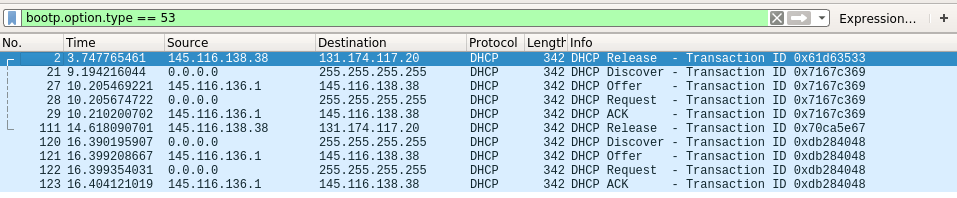
\includegraphics[width=\linewidth]{screenshots/dhcp}

\begin{enumerate}[a]
	\item %a
	The Ethernet address of my host is 18:cf:5e:15:89:47. It can be found in the Ethernet frame.

	\item %b
	The DHCP request is almost the same as the DHCP discover message except that it contains a DHCP Server Identifier with the IP of the DHCP server.

	\item %c
	The DHCP server's IP is 131.174.117.20.

	\item %d
	\item %e
	\begin{tabular}{|c|c|}
		\hline
		Action & Transaction ID\\\hline
		Release 1 & 0x61d63533\\\hline
		Request 1 & 0x7167c369\\\hline
		Release 2 & 0x70ca5e67\\\hline
		Request 2 & 0xdb284048\\\hline
	\end{tabular}

	Each transaction (set of messages that belong together) has an ID to keep track of the transaction should there be more than one.

	\item %f
\end{enumerate}

\section{} %2
\begin{enumerate}
	\item %1
	\begin{tabular}{|c|c|}
		\hline
		Interface & IP\\\hline
		A & 192.168.1.1\\\hline
		B & 192.168.1.2\\\hline
		C & 192.168.2.1\\\hline
		D & 192.168.2.2\\\hline
		E & 192.168.3.1\\\hline
		F & 192.168.3.3\\\hline
	\end{tabular}

	\item %2
	To answer this question we need to know the MAC addresses of the interfaces on the routers. I assume addresses $X_1$, $X_2$ for the right router and $Y_1$, $Y_2$ for the left router.

	\begin{enumerate}
		\item E sends a datagram to (192.168.1.2, $X_2$)
		\item $X_2$ forwards the datagram to (192.168.1.2, $Y_2$)
		\item $Y_2$ forwards the datagram to (192.168.1.2, B)
	\end{enumerate}

	\item %3
\end{enumerate}

\section{} %3

\section{} %4
\begin{enumerate}
	\item %1
	\item %2
	\item %3
	\item %4
	\item %5
\end{enumerate}

\section{} %5
\begin{enumerate}[a]
	\item %a
	I started the 3 hosts with these commands:
	\begin{lstlisting}
# terminal
vstart PC1 --eth0=A
vstart PC2 --eth0=A
vstart PC3 --eth0=A

# for PC1
ifconfig eth0 1.0.0.1 up
# for PC2
ifconfig eth0 1.0.0.2 up
# for PC3
ifconfig eth0 1.0.0.3 up
	\end{lstlisting}

	Then I ran arp on each machine. All ARP tables were empty:

	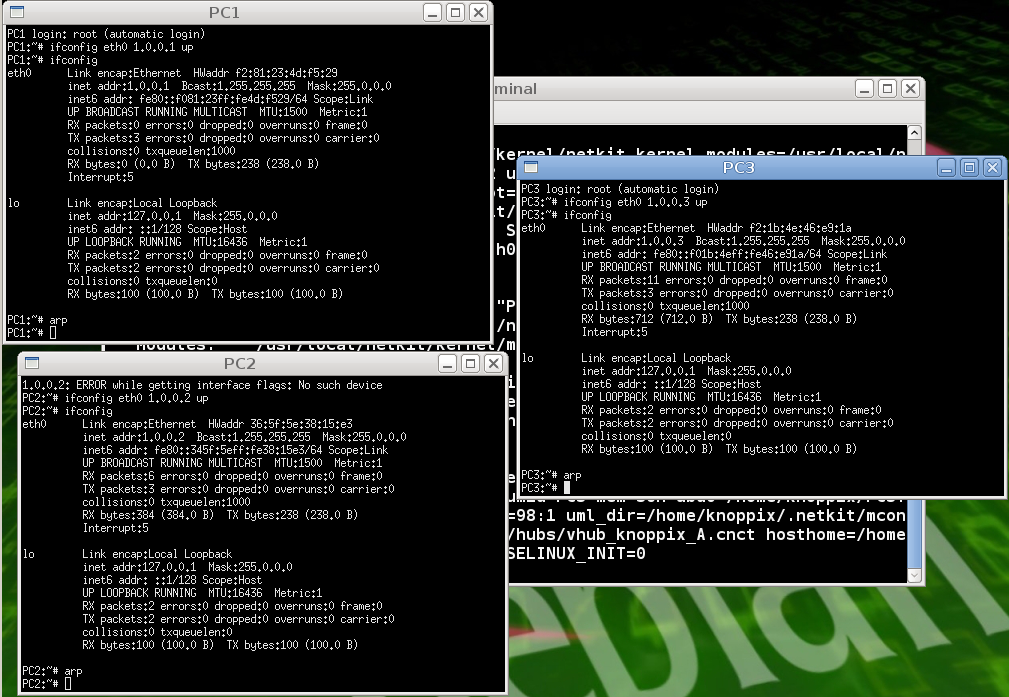
\includegraphics[width=\linewidth]{screenshots/screen1}

	Then I pinged PC2 from PC1 and ran arp again:

	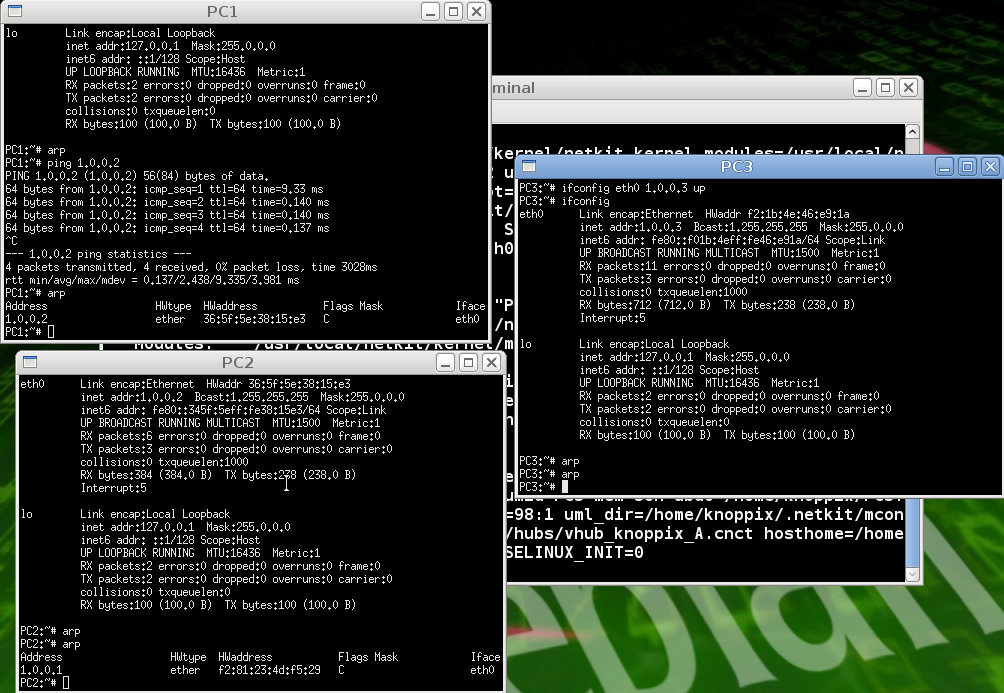
\includegraphics[width=\linewidth]{screenshots/screen2}

	PC1 now knows about the MAC address of PC2 and vice versa. PC3 still has an empty ARP table.

	\item %b
	To ping PC2, PC1 needs to know PC2's MAC address. Because PC1's ARP table is empty it broadcasts an ARP query to the IP of PC2. PC2 receives the broadcast with PC1's IP and MAC and adds it to the ARP table. Next PC2 responds to the ARP query. PC1 receives PC2's response and adds an entry for PC2 to the ARP table.

	PC3 isn't involved in the transaction and does not get any updates. It receives the ARP broadcast from PC1 but does not respond to it because it does not match the IP of PC2.

	\item %c
	I spoofed PC2's MAC address from PC3:
	\begin{lstlisting}
arpspoof -i eth0 1.0.0.2
	\end{lstlisting}

	Next I pinged PC2 from PC2 and looked at the ARP tables again:

	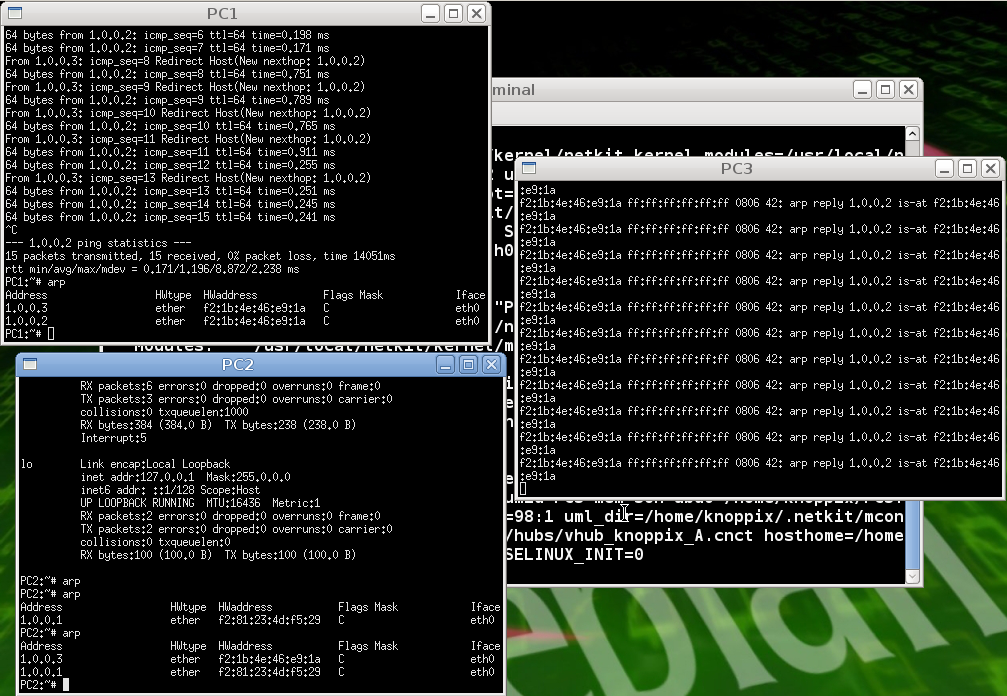
\includegraphics[width=\linewidth]{screenshots/screen3}

	PC1 now has two entries (for PC2 and PC3) with the MAC address of PC2. The first entry is correct, the second one was spoofed by PC3.

	PC2 still has the entry for PC1 but now has an additional entry for PC3 but with the MAC of itself (PC2), that was spoofed by PC3.

	PC3 know has a correct ARP entry for PC2 because it looked up PC2's MAC address to spoof it.

	\paragraph{What happened?}
	PC3 started an ARP lookup for the IP 1.0.0.2 which belongs to PC2. It received the MAC address of PC2 and began sending out ARP responses with the MAC of PC2. PC2 and PC1 received those responses and added the spoofed entry to their ARP tables.
\end{enumerate}

\end{document}
